\documentclass{article}
\usepackage[utf8]{inputenc}
\usepackage{graphicx}
\usepackage{hyperref}
\usepackage{amsmath}
\usepackage{xcolor}

\title{PiBrain Documentation}
\author{Andrew M. Evans, Leo P. Janzen}
\date{July 2021}

\begin{document}

\maketitle

\tableofcontents

\section{Introduction}
This document aims to give a complete outline of both the software and hardware used in the PiBrain v0.1-alpha. The documentation will also act as an installation guide, and a place to detail potential future projects. The \LaTeX\ source code for this PDF will be included in the PiBrain repository on GitHub, it is highly recommended that any future work on PiBrain be document here.\\

\subsection{Description}
PiBrain is a raspberry pi operated replacement for PLC on the MK-VII thermal evaporator system. The software is written in primarily python 3.8.0, with some auxiliary scripts written in bash. The hardware is a simple 24V to 3.3V logic conversion using ISOs and relays.\\

\subsection{Purpose}
The main purpose of PiBrain is to provide an easily modifiable platform for controlling the MK-VII thermal evaporator system. Section~\ref{section:future} focuses on future applications/ideas for what the system could be capable of. The primary focus of this document will be establishing how the hardware was built, and how the software was written with respect to the manual mode.
\subsection{Contact information}

To contact the original creator (Andrew) please use the following resources:
\begin{itemize}
    \item Email: evansa@sonoma.edu (only good till 2023)
    \item Alternate email: andrew.m.evans1989@gmail.com
    \item Discord: Andrew Evans\#4366
\end{itemize}
To contact the creator of the hardware (Leo) please use the followiing 
\begin{itemize}
    \item Email: lpjanzen@ucdavis.edu
\end{itemize}


Responses wont be instantaneous, but we will try and get around to it!

\section{Software}
\label{section:software}
This section will detail all current pieces of the code along with idea behind the organization and structure of the code. The code is broken up into three categories: bash scripts, state machine, and main. The general idea of the code is that the bash scripts do the operating system level work (automated startup, file clean up, etc see Section~\ref{section:bash}), the state machine does the ``organizational'' work of the software (running the main logic tree which includes the idle loop see Section~\ref{section:state}), and lastly main which contains the hardware interfacing code (see Section~\ref{section:main}). There are some aspects of this layout which could\footnote{most likely should be changed} be changed in the future (see Section~\ref{section:future}).

\subsection{Bash scripts}
\label{section:bash}
Currently there are two bash scripts: clear\_run\_cache.sh, and startCode.sh. Both scripts are incredibly simple and act as a way of automatically running system commands

\subsubsection{Clearing output cache}
The first script is responsible for clearing the outputfile cache. During run time the code will produce an outfile file which logs changes while the code is running. For example if the vent command is called then it will log the vent command along with a time stamp, see Figure~\ref{fig:logfile}. 
\begin{center}
    \begin{figure}[h!]
      
\includegraphics[scale=0.4]{image1.png}
      \caption{Example log file}
      \label{fig:logfile}
    \end{figure}
\end{center}


After the runs the bash script will clear this file \textbf{NEED TO ADD OPTION FEATURE FOR THIS}. default setting will be to clear the run cache after run.\\


\subsubsection{Automated startup}
The other script, startCode.sh, is responsible for starting the code on the boot up of the raspberry pi. \textbf{NEED TO ADD FILE TO BOOT DIRECTORY}. The hope is that SSH connection to the pi would be minimal, and that in most of the use cases the raspberry pi could automatically start and clear run caches without the need for human intervention, see Section~\ref{section:raspi}.

\subsection{State machine}
\label{section:state}
Statemachine.py is the organizational backbone of the code fig~\ref{fig:state}. Any defined command should run through the state machine if possible, however the definitions should occur outside the state machine\footnote{Again, this is something that was not done super well and will be addressed in Section~\ref{section:future}}\\ \textbf{EDIT PICTURE OF STATE MACHINE}\

\begin{center}
    \begin{figure}[h!]
      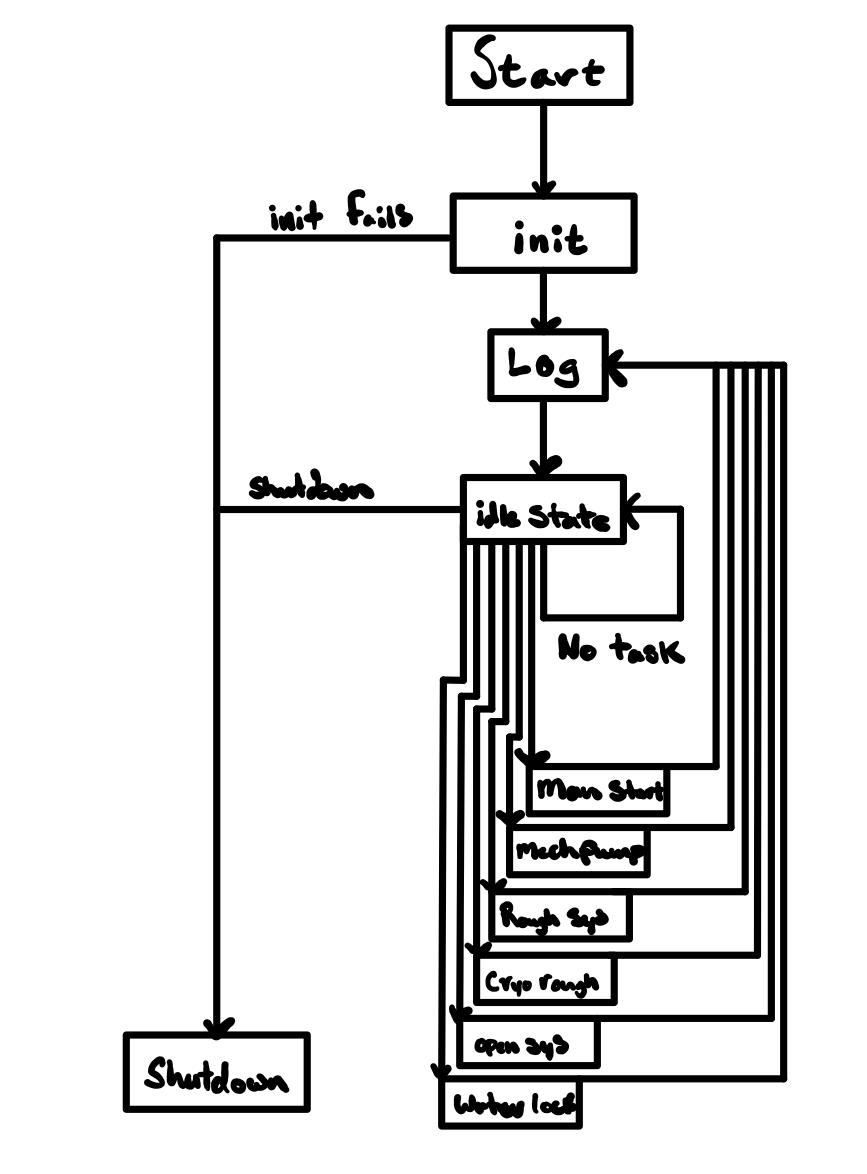
\includegraphics[scale=0.4]{IMG_0432.jpg}
      \caption{State machine logic}
      \label{fig:state}
    \end{figure}
\end{center}

\subsubsection{Imports}
\label{section:imports_sm}
The imports are used for getting the date and time for the log file, and for pausing the script. The main reason for wanting a script pauses is that the main loop of the state machine is effectively an infinite loop. Without the pause feature the loop runs much faster than a user could ever hope to make inputs. Documentation for the modules: \href{https://docs.python.org/3/library/datetime.html}{datetime}, 
\href{https://docs.python.org/3/library/time.html}{time}\footnote{time and datetime are hyperlinks, click to see the documentation}\\

\subsubsection{State machine class}
The state machine itself is defined as an object in the code. It has two attributes: outputfile, and inputfile. These names make the purpose pretty obvious, but for those who haven't caught on, it's for setting the input and output file paths. The output file is what the log is written into, and the input file is designed for simulating the machine. The input feature will likely be changed or removed before the final draft of this document \textbf{YOU HEAR THAT? YOU SHOULD EDIT THIS OUT LATER}. The state machine itself has three methods: write\_to\_log, idleTaskCheck, and idle\_state. These methods will be discussed in more detail below.

\subsubsection{write\_to\_log}
\label{section:logwrite}
This method looks at the return codes thrown by the different tasks and using this determines what message to print into the log file. Tasks return a three-tuple of which the first two elements are booleans, and the last is a string. The general form of the tuple is:\\
$$\left(\text{Expected exit}, \text{ Task completed},\text{ Name of task}\right)$$
Table~\ref{table:returnl} shows what the different combinations of trues and falses yield. 

\begin{itemize}
    \item \textbf{Key} to table~\ref{table:returnl}:\\
    OK -the system completed the task\\
    NC -the task didn't change\\
    NA -not applicable (combination not set)\\
    FAIL -an error has occurred\\
\end{itemize}

\begin{table}[h!]
\centering
    \begin{tabular}{c|c|c}
      & T  & F    \\ \hline
    T & OK & NC   \\ \hline
    F & NA & FAIL 
    \end{tabular}
\caption{Return statement logic}
\label{table:returnl}
\end{table} 


While this system works it is definitely another point in the code which should be reworked in the future, see Section~\ref{section:future}.
\subsubsection{idleTaskCheck}
This method simply compares the last task with the current task looking to see if there had been a change in the task's state. If the task's state had changed then the function writes this to the log file. This was designed so that the log file would only report changes in task, reducing the overall space used on the raspberry pi.

\subsubsection{idle\_state}
the idle\_state method is the heart of the state machine. The method is responsible for all code that is updated every loop. There are eight inputs to this method (excluding the self input). All the inputs that start with ``task'' are the actual logical functions defined in main passed into the method. The update\_pins input is the pin reading function defined in main called readPinsLoop. The first variable (called delay) inside the idle loop gives the ability to set the delay on the actions in the loop in seconds. During the loop the state machine pauses and waits one second between each prompt. This is to ensure that the code is not overworking the raspberry pi. After the delay is set the code initializes all the ``task\#\_last'''s this is done so that the idleTaskCheck method will work on the first loop, and so that the code will write all of task's states to the log file upon startup.\\
After the initialization of the idle loop the variable machine\_on is set to true and the code enters the while loop. This loop is infinite and will only close when machine\_on gets set to false. This can happen in only two cases. \\

\textbf{Case 1:} If any of the tasks return statements throw a first element false, this is defined as an emergency halt. For more information on the tuple edit code system see Section~\ref{section:logwrite}. \\

\textbf{Case 2:} If the stop pin \textbf{MIGHT CHANGE} is called. \\

Case 1 can only be called if the update\_pins function doesn't return a false. False is returned from the function if case 2 will happen. This was designed this way so that if a stop code is called it wont try and run all the tasks. This method could be improved, see Section~\ref{section:idleE}.

\subsection{Main}
\label{section:main}
Main is where the code is run from and where the definitions of the pins and processes are. If additional logic is added to the code the definitions should be put in main. In the future the code written in main could be split into two separate files so that the definitions are done in another file see Section~\ref{section:mainsplit} for more detail.

\subsubsection{Manual mode}
The code currently supports a manual mode. This means that the user must toggle switches on the actual deposition machine itself, which sends signals to the raspberry pi, and then finally the pi decides if it is ``safe'' to turn on the called process. This means that without explicitly telling the pi what to do nothing will happen. This system is capable of being fully automatic, for more detail on this project please see Section~\ref{section:auto}.

\subsubsection{Imports}
This piece of code currently imports the following packages: time, datetime, StateMachine, and os. For more information on time, and datetime see Section~\ref{section:imports_sm}. The package Statemachine is the code described in Section~\ref{section:state}. The last package imported, as mentions, is os. os lets the user interface with the operating system. The documentation can be found here: \href{https://docs.python.org/3/library/os.html}{os}.

\subsubsection{bcolors}
This class allows for text color to be set by adding attributes of this class to strings. This code is an adaptation of the code found at the following \textbf{\href{https://stackoverflow.com/questions/287871/how-to-print-colored-text-to-the-terminal}{source}}. An example of the code being used can be found in figure~\ref{fig:bcolors}.

\begin{center}
    \begin{figure}[h!]
        print(bcolors.FAIL+``Oh god the computer is on fire''+bcolors.RESET)\\
        $>$$>$$>${\color{red}Oh god the computer is on fire}
      \caption{Example use of bcolors}
      \label{fig:bcolors}
    \end{figure}
\end{center}

Note to the reader, if bcolors.RESET isn't called the code will remain in the last color you set, even after the code is exited.


\subsubsection{IO\_Devices}
The IO\_Devices class was build to hold the structure of an input or output device as one object. The object has 5 attributes: name, state, pin, ras\_pin, and  IO\_type.

\begin{itemize}
    \item name - what the pin corresponds to, see Table~\ref{table:PLClogic}
    \item state - whether the pin is high or low 
    \item pin - the number of the pin according to Table~\ref{table:PLClogic}
    \item ras\_pin - number of pin on the raspberry pi
    \item IO\_type - whether the pin is an input or output
\end{itemize}
The \href{https://www.w3schools.com/python/python_classes.asp}{initialization}\footnote{For more information on classes and initialization click the word initialization} of IO\_Devices also has some logic for choosing whether to set the GPIO pin to be read or write.\\

The first method (other than init) is the setHigh method. This method sets output pins high. It first checks to see if the the pin is an input or output pin and then if it is an output pin then it checks if it is already set high. If the pin is already set high then it prints that it is maintain high, if it isn't already set high it prints that it is setting the pin high and then sets the state of the pin to high. If the pin is an input it does not set it high and prints a warning that you are attempting to set a read pin. This could more optimally be forced by creating an IO\_Device parent class with input and output children classes where the input class would not contain the setHigh and setLow methods, see Section~\ref{section:IOclassedit}.\\

Next is the setLow method. This method serves the exact same purpose as the setHigh method but sets the pin low. These two methods could technically be done in one method taking an argument for setting high vs low, however, this was decided against to improve readability.\\

\subsubsection{Tasks}
The tasks are the main functions which the machine communicates to the state machine. Potential changes to this organization are discussed in Section~\ref{section:mainsplit}. The general idea is that the tasks contain simple logic conditions which result in setting pins using the setHigh/Low methods and then the task returns a three-tuple as discussed in Section~\ref{section:logwrite}. To see the logic for each task see Fig~\ref{fig:ladder}. \\

There are three task that do show up on Fig~\ref{fig:ladder}. These tasks do not correspond to a piece of the physical machine, but rather they are used for lower level actions. The three functions are: readPinsLoop, shutdownSys, and system\_status. \\

readPinsLoop checks a text file to see if the pin in the file is set to true. This will be changed in the final build to actually read from the pins!\\

shutdownSys sets all the output pins to low. This done to not draw power while the system is off, and also make the raspberry pi safe to handle once the system is shutdown.\\

system\_status is a debugging tool used to quick output the status of all the pins. This function is only used when testing the code, but with some minor modification could print to a new text log file acting as a more powerful debugging tool see Section~\ref{section:systemstatchange}.

\subsubsection{Pin definitions}
\label{section:pin_def}
The pins are fully defined in the code, however for the sake of convenience their names and numbers will be listed in Table~\ref{table:pin_def_t}. In the current build two pins remain free (20, and 21 on the raspberry pi).
\begin{table}[h!]
\centering
    \begin{tabular}{|l|l|l|l|}
    \hline
    Name  & Input/Output& Pin number & GPIO number    \\ \hline
    Start & Input & 0000 & 26   \\ \hline
    Stop & Input & 0001 & 19 \\ \hline
    Crossover & Input & 0002 & 13 \\ \hline
    Auto & Input & 0003 & 06 \\ \hline
    On\_Reset & Input & 0004 & 05 \\ \hline
    Manual & Input & 0005 & 00 \\ \hline
    Vent & Input & 0006 & 11 \\ \hline
    Rough\_S2 & Input & 0007 & 09 \\ \hline
    COM & & & \\ \hline
    & & & \\ \hline
    HI\_VAC\_Valve & Input & 0008 & 10 \\ \hline
    Cryo\_Rough & Input & 0009 & 22 \\ \hline
    Cryo\_Purge & Input & 0010 & 27 \\ \hline
    Vacuum\_In & Input & 0011 & 17 \\ \hline
    Rough\_SW & Input & 0012 & 04 \\ \hline
    Water\_Lock & Input & 0013 & 03 \\ \hline
    Vent\_Auto & Input & 0014 & 02 \\ \hline
    -NONE- & Input & 0015 & 14 \\ \hline
    COM &  &  &  \\ \hline
     &  &  &  \\ \hline
    OUT0 & Output & 0500 & 14 \\ \hline
    OUT1 & Output & 0501 & 15 \\ \hline
    OUT2 & Output & 0502 & 18 \\ \hline
    OUT3 & Output & 0503 & 23 \\ \hline
    OUT4 & Output & 0504 & 24 \\ \hline
    OUT5 & Output & 0505 & 08 \\ \hline
    OUT6 & Output & 0506 & 07 \\ \hline
    OUT7 & Output & 0507 & 01 \\ \hline
    COM & & & \\ \hline
    & & & \\ \hline
    OUT8 & Output & 0508 & 12 \\ \hline
    OUT9 & Output & 0509 & 16 \\ \hline
    -NONE- & Output & 0510 & 20 \\ \hline
    COM & & & \\ \hline
    & & & \\ \hline
    -NONE- & Output & 0511 & 21 \\ \hline
    COM & & & \\ \hline
    & & & \\ \hline
    \end{tabular}
\caption{PLC codes and GPIO numbers grouped by COM}
\label{table:pin_def_t}
\end{table} 

\section{Hardware}
There are two main pieces of hardware that make up the PiBrain, there is the raspberry pi, the ``Brain'', and there is the PCB, the ``nervous system''. This section will aim to cover the specifics of each. Attached with this PDF there will be schematics of the hardware, with CAD files. The main goal of this is to have easy documentation to help with repairs and future work. There will also be a subsection detailing the computer that the PiBrain is replacing and hardware which PiBrain will control.

\subsection{Overview}
This board interfaces between a Cooke MK-VII Vacuum Deposition Machine and a Raspberry Pi Zero w. It has been designed to replace the Omron Sysmac C20, and thus copies the input/output schema of the C20.\\

Input COMs should be connected to +24V. Raspberry Pi inputs are \textbf{normally high} (3.3V). When an IN is connected to ground, the corresponding LED will illuminate and the corresponding Raspberry Pi pin will be pulled low (0V).\\

When Raspberry Pi outputs are low (0V), the corresponding OUT will be open circuit. When the Raspberry Pi output goes high (3.3V), the corresponding LED will illuminate, and the corresponding OUT will be connected to a COM via a relay.\\

\textbf{
NOTE: Internal and external inputs and outputs are completely isolated from each other. The mounting hole in the upper right (labeled GND) is connected to internal ground and can be connected to external ground if desired.}\\


\begin{table}[h!]
\centering
    \begin{tabular}{|l|r|c|}
    \hline
    Name  & Value & Units   \\ \hline
    Input Voltage ($\text{V}_{\text{COM-INX}}$)  &  &    \\ \hline
    Maximum operating & -15 & V\\ \hline
    Typical operating & -24 & V \\ \hline
    Minimum operating & -30 & V \\ \hline
    Absolute Maximum &  30 & V \\ \hline
    Absolute Minimum & -30 & V \\ \hline
    & & \\ \hline
    Input current $\text{I}_\text{INX}$ & & \\ \hline
    Typical forward (-24V) & 10 & mA \\ \hline
    & & \\ \hline
    Maximum Output Switching Voltage & 30 & V \\ \hline
    & & \\ \hline
    Output Current & & \\ \hline
    Maximum Per Output & 5 & A \\ \hline 
    Maximum Per COM & 16 & A \\ \hline

    \end{tabular}
\caption{Electrical characteristics}
\label{table:elec_char}
\end{table} 

\subsection{Raspberry pi}
\label{section:raspi}
The ``Brain'' of this project so to speak is a \href{https://www.raspberrypi.org/products/raspberry-pi-zero-w/}{ Raspberry Pi Zero w}\footnote{Click for a link to the website}. This controller runs all the software described in Section~\ref{section:software}. Table~\ref{table:pin_def_t} contains all the information on how the GPIO pins on the raspberry pi correspond to the functions in the software.

\subsection{PCB}
This section will give detail on the PCB which the raspberry pi is attached to. This Piece of hardware is designed to allow the raspberry pi to communicate with the deposition machine without being on a 30V circuit.
\begin{center}
    \begin{figure}[h!]
      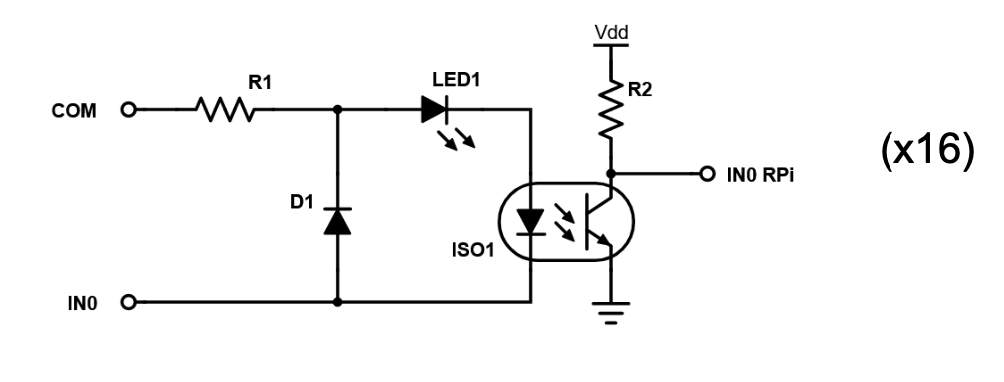
\includegraphics[scale=.8]{inputschem.png}
      \caption{Input schematic. COM is connected to +24V. When IN0 goes low, LED1 and ISO1 will turn on, pulling down IN0 RPi to 0V. When IN0 is high or disconnected, IN0 RPi will be pulled up to 3.3V by R2.}
      \label{fig:input_schem}
    \end{figure}
\end{center}



\begin{center}
    \begin{figure}[h!]
      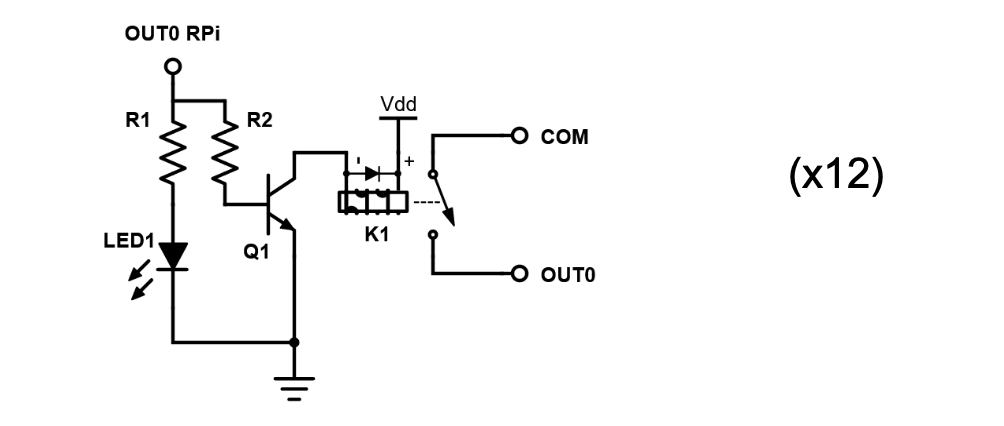
\includegraphics[scale=.9]{outputschem.png}
      \caption{Output schematic. When OUT0 RPi goes high (3.3V), LED1 will light and Q1 will actuate K1, connecting OUT0 to COM.}
      \label{fig:output_schem}
    \end{figure}
\end{center}


\subsection{Case}

\subsection{Deposition machine}

\subsubsection{PLC}
This is a direct copy of what was used to run the PLC, and what the PiBrain was adapted from. \textbf{Disclaimer:} This table is not fully understood\footnote{That is not a joke}.

    \begin{table}[h!]
    \scalebox{0.7}{
        \begin{tabular}{|l|l|l|l|l|l|l|l|}
            \hline
            Input 0 CH & IN & Terminal \# & Input device & Output 5 CH & Out & Terminal \# & Output device  \\ \hline
            0 PB3 & 0000 & A0 & START (PB3) & 0 & 0500 & A10 & AUTO  \\ \hline
            1 PB4 & 0001 & B0 & STOP (PB4) & 1 & 0501 & B10 & MANUAL  \\ \hline
            2 & 0002 & A1 & CROSSOVER & 2 & 0502 & A11 & VENT  \\ \hline
            3 S8 AUTO & 0003 & B1 & AUTO (S8) & 3 & 0503 & B11 & R VAL?  \\ \hline
            4 PB1 & 0004 & A2 & ON/RESET & 4 & 0504 & A12 & -NONE-  \\ \hline
            5 S8 Manual & 0005 & B2 & MANUAL & 5 & 0505 & B12 & CRYO ROUGH  \\ \hline
            6 S1 & 0006 & A3 & VENT & 6 & 0506 & A13 & CRYO PURGE  \\ \hline
            7 S2 & 0007 & B3 & ROUGH (S2) & 7 & 0507 & B13 & HI VAC?  \\ \hline
            8 S3 & 0008 & B4 & HIGH-VAC VALVE (S3) & 8 & 0508 & B14 & WATER LOCK  \\ \hline
            9 S4 & 0009 & A5 & CRYO ROUGH (S4) & 9 & 0509 & A15 & ROUGH PUMP  \\ \hline
            10 (S5) unmarked & 0010 & B5 & CRYO PURGE & 10 & 0510 & B15 & -NONE-  \\ \hline
            11  & 0011 & A6 & VACUUM IN & 11 & 0511 & B16 & -NONE-  \\ \hline
            12 S6 & 0012 & B6 & ROUGH SW (S6) &  &  &  &   \\ \hline
            13 & 0013 & A7 & WATER LOCK &  &  &  &   \\ \hline
            14 PB5 & 0014 & B7 & VENT-AUTO &  &  &  &   \\ \hline
            15 & 0015 & A8 & -NONE- &  &  &  &   \\ \hline
        \end{tabular}
        }
    \caption{Return statement logic}
    \label{table:PLClogic}    
\end{table}

\begin{center}
    \begin{figure}[h!]
      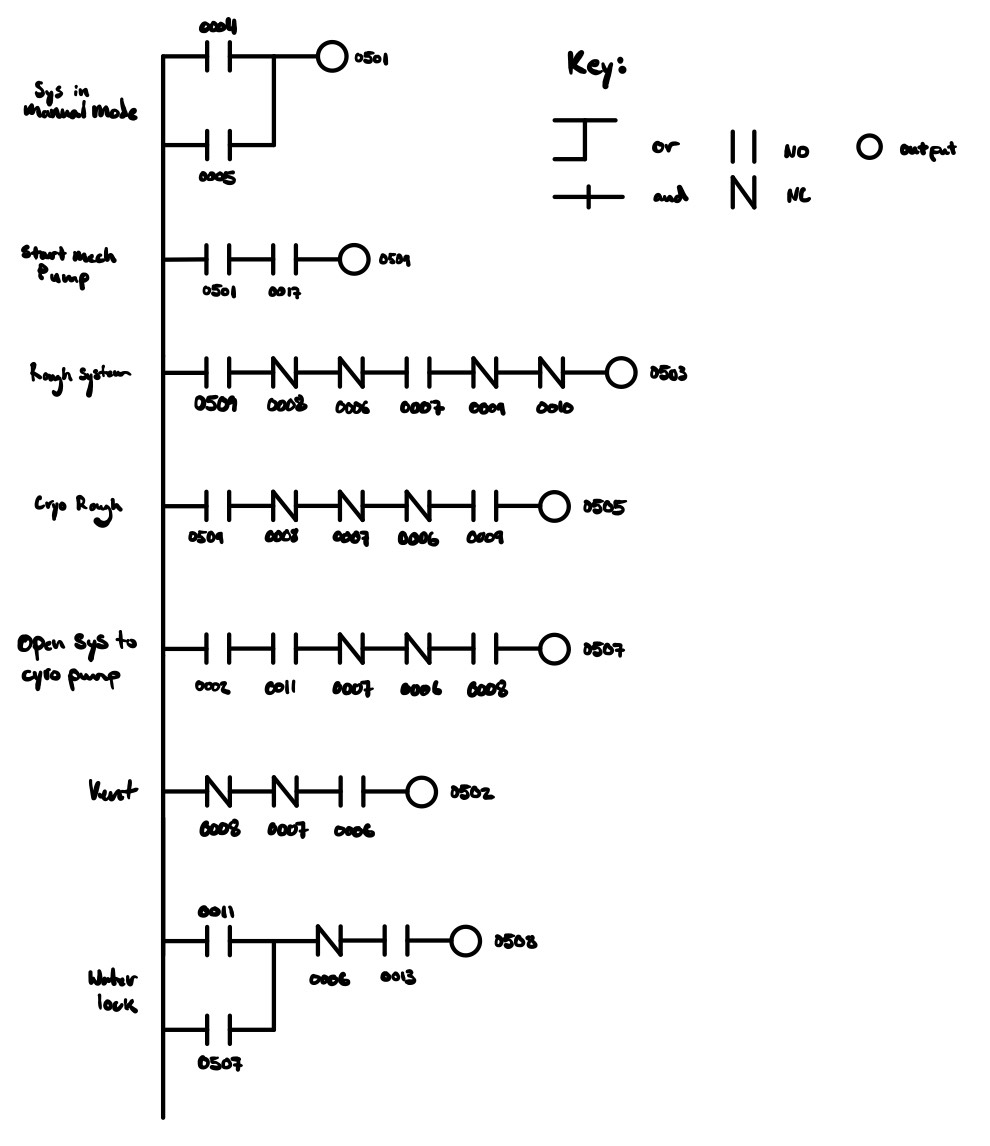
\includegraphics[scale=0.4]{IMG_0434.jpg}
      \caption{Ladder logic for the PLC}
      \label{fig:ladder}
    \end{figure}
\end{center}
For more information on what the codes in Fig~\ref{fig:ladder} please see Section~\ref{section:pin_def}

\section{Installation}
At the time of this documents creation the PiBrain is not installed on the deposition machine. This task will be left as work for the next person to take on this project\footnote{I hope that you enjoy your work on PiBrain :)}. The installation should happen in two parts: fitting, and wiring. The PiBrain will be put inside a case which will have mounting holes, bolts will be fit through the mounting holes into newly drilled holes in the deposition machine\footnote{With some clever design the PiBrain case could attach to the deposition machine in the same way that the PLC attached to the machine!}. The wiring will relatively trivial compared to the rest of the process as long as the user labels the wires before they remove them from the original hardware.

\section{Future work}
\label{section:future}
There is a lot of work that still needs to be done and that could be done. This software and hardware

\subsection{Combination of bash scripts with python}
\label{section:picombo}

\subsection{write\_to\_log rework}

\subsection{Idle exit}
\label{section:idleE}

\subsection{Main file split}
\label{section:mainsplit}

\subsection{Deposition controller pi}

\subsection{Web interface}

\subsection{GUI interface}

\subsection{Automatic mode}
\label{section:auto}
probably will need another pi, blah blah blah, pi network....

\subsection{IO\_Device class change}
\label{section:IOclassedit}

\subsection{Allowing for hard exits}
no code currently shutdown the machine completely. This should be changed.

\subsection{System file log}
\label{section:systemstatchange}
Creating a logging system with the system\_status function that is stored locally on the pi.
\end{document}
